%Move from macro to micro, citing from oldest references to the most recent

%What it is: 
%–Overview of previous work in the field 
%– What’s the big picture?
%–Explanation of how your work addresses the gap in the field
%–Enough technical details for the reader to understand your project
%–Explanation of importance/impact of your work 

%What you need to show: 
%–You understand what’s going on in your field, and how your work fits into that. 
%–You have the authority to say your research is important/novel. 

%Can be helpful to... 
%–Restate your hypothesis 
%–Briefly mention an experimental overview (just enough to lead the reader into your Project Plan)

Section 2 contains a brief background to Neural Networks (NNs) and RNNs. This will be followed by related work in the field of Exoplanet Transit detection and vetting. 
\subsection{Neural Networks}
Machine Learning (ML) is a type of computer algorithm that is used to predict certain outputs based on the input data. The heuristics of what to learn from the data are automatically identified by the ML model using a process called \emph{"Training"}. For a given set of inputs, the training process adjusts model parameters while minimizing the difference between the predicted (mathematically calculated) output of the model and the actual output. This difference is calculated by a cost function.\\

Deep Learning is a subset of ML which uses mathematical sub-units called neurons. Each of these neurons are arranged in layer like format, where every neuron from one layer is connected to every other neuron in the next layer. The connections between these neurons are multiplicative factors called weights and each neuron has an additive factor, called bias, leading to their configuration as
\begin{center}
$a_i = f(W_i * x\textsubscript{i-1} + b_i)$
\end{center}

where $a_i$ is the output of neuron layer \emph{i} when $x\textsubscript{i-1}$ is the input from the previous (\emph{i-1})$^{th}$ layer neurons and $f()$ is an activation function which induces non-linearity. Figure 1 shows a Fully Connected (FC) Network.

%Figure
\begin{figure}[H]
    \centering
    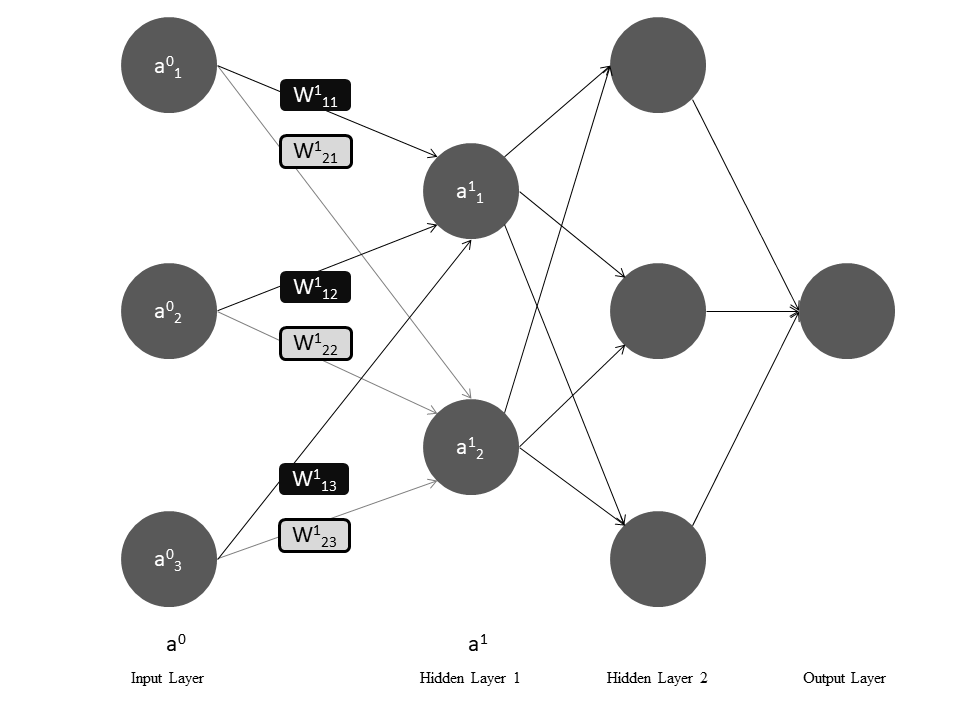
\includegraphics[scale=0.35]{Images/ANN.png}
    \caption{A Fully Connected Neural Network with 2 Hidden Layers. Connections weights are shown between Input layer and Hidden layer 1}
    \label{fig:ANN}
\end{figure}

The backpropagation algorithm changes these weights and biases of the neurons in order to minimize the cost function. Cross Entropy loss is calculated as the cost function for binary classification problems. In order to minimize the cost, we take gradient of the cost with respect to the parameters of the model and equate it to 0. This indicates the iterative updation of parameters till a minima for the cost is reached.\\

Convolutional Neural Networks are a class of neural networks which use convolution (or discrete cross-correlation) operation on the input with a kernel/filter at the convolution layer. The resulting \emph{feature map} is fed to pooling layer which aggregates regions in the neighbouring proximity using mean or maximum values, the output of which is finally fed to a fully connected layer for the prediction. The output of the convolutional layer, or the feature map is given by \\
\begin{center}
    $a_i^{(l)} = f(\sum_{k=1}^K w_i^{(k,l)} * a_{i-1}^{(k)} + b_i^{(l)})$
\end{center}
where the $K$ vectors of length $n_{i-1}$ are input to the $i^{th}$ layer (k=1,2, ..., K) given by $a_{i-1}^{(k)}$, L is the output number of vectors (l=1,2, ...,L) given by $a_i^{(l)}$, $f()$ is the activation function, $*$ is the convolution function, $w_i^{(k,l)}$ is the weight array acting as a filter or kernel and $b_i^{(l)}$ are the bias vector.


\subsection{Recurrent Neural Networks}
RNNs feed the output of the network back as an input to the network. This allows them to retain information, identify patterns and establish temporal connections, which is suitable for time-series applications.
\begin{figure}[h]
    \centering
    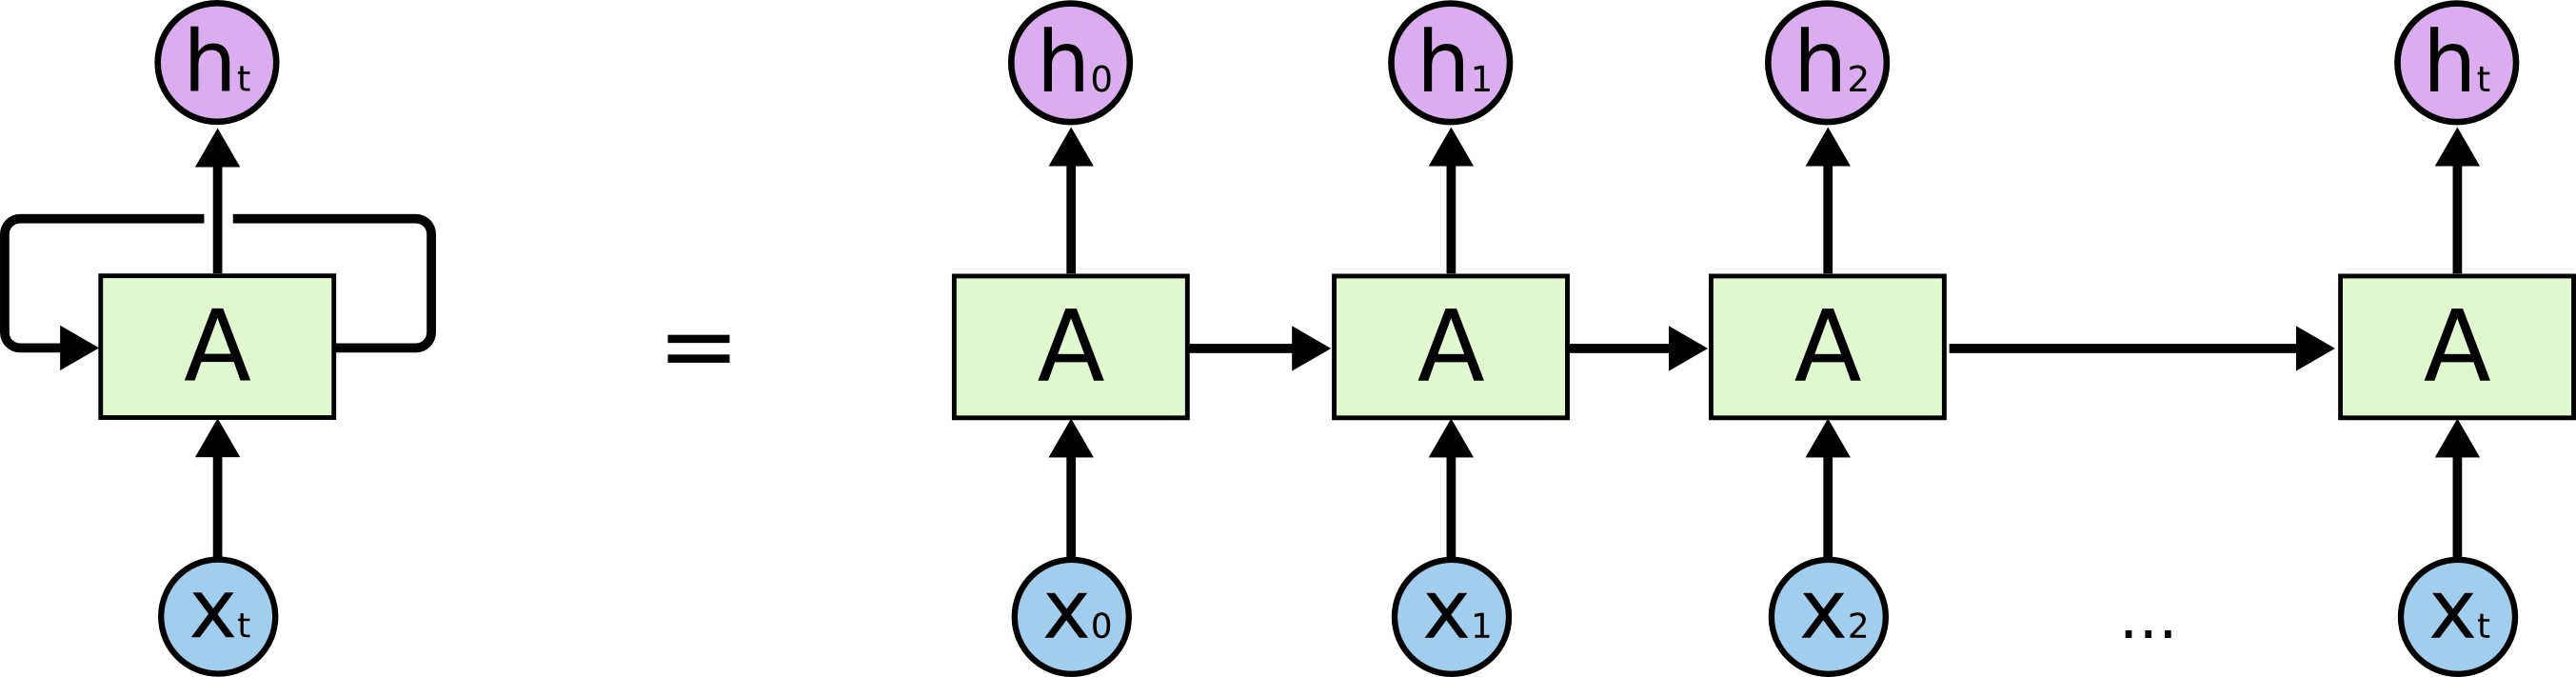
\includegraphics[scale=0.3]{Images/RNNs_1.png}
    \caption{A Recurrent Neural Network. The looped layers are shown unrolled here. \emph{Source}: \href{https://colah.github.io/posts/2015-08-Understanding-LSTMs/}{\textit{Understanding LSTM Networks, Colah 2015}}}
    \label{fig:RNN}
\end{figure}
Long Short Term Memory Networks are a type of gated RNNs that can learn long term dependencies between the data points by removing or adding certain information. A Cell-state flows through the LSTM cells which holds the long term memory. The information which we need to remove is decided by the first sigmoid gate. The second sigmoid gate in conjecture with $tanh$ of the previous state's output decides what we keep in the cell state. This cell state then factors in with a $tanh$ to the current state's output.
\begin{figure}[h]
    \centering
    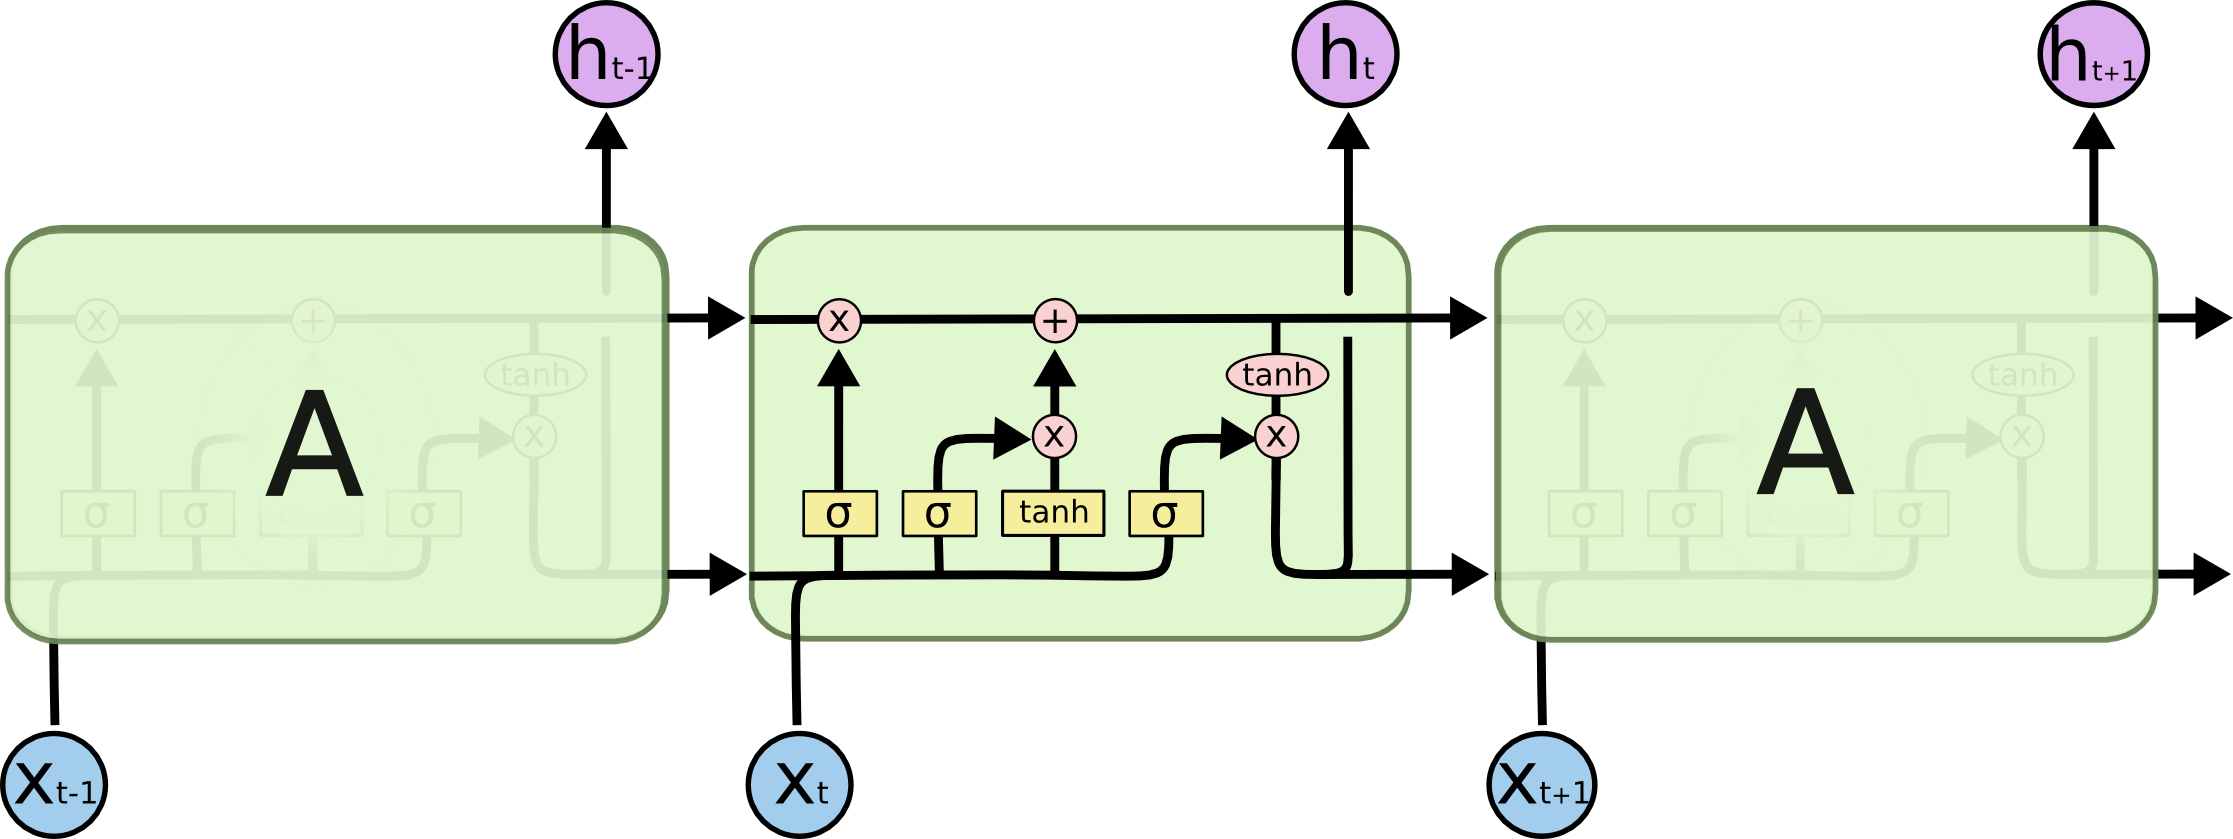
\includegraphics[scale=0.35]{Images/LSTM.png}
    \caption{Simplified architecture of Long Short Term Memory Network. \emph{Source}: \href{https://colah.github.io/posts/2015-08-Understanding-LSTMs/}{\textit{Understanding LSTM Networks, Colah 2015}}}
    \label{fig:LSTM}
\end{figure}
\vspace{-0.3in}
\subsection{Exoplanet Transit Detection}
Transit detection for exoplanets is a field involving space-based high precision photometry. A dip in the stellar flux/brightness indicates a transit (passage of an object between telescope's field of vision and the star). We record the stellar brightness over a fixed time span and the resulting flux time series is called a \emph{Light Curve}. The first transiting exoplanet was detected by Charbonneau et al. in 1999 \cite{char}. \\
\begin{figure}[h]
    \centering
    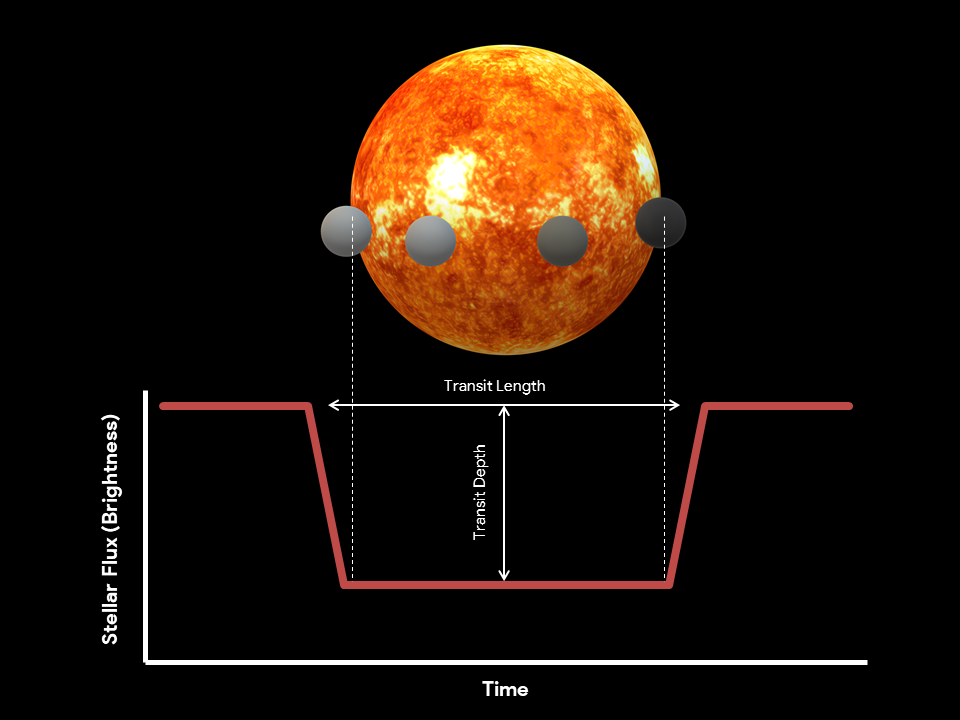
\includegraphics[scale=0.3]{Images/Transit.png}
    \caption{Stellar light curve plotted against a planet transiting it's host star}
    \label{fig:Transit}
\end{figure}

Space based telescope missions, like the Kepler, has a pipeline called Science Processing Pipeline \cite{2dcnn} which detects these transits in the collected noisy data. The pipeline first calibrates the captured photometric pixels or the TPF (Target Pixel File) and performs fixed-aperture photometry to remove instrumental errors. The transit events are detected in the light curves and these Threshold Crossing Events (TCEs) are filtered in. The TCEs can be Planet Candidates (PC), Astrophysical False Positives (AFP) caused by Eclipsing Binaries (EB) or Background Eclipsing Binaries (BEB), Non Transiting Phenomena (NTP) as caused by star-spots, pulsations or stellar flares, or Unknown phenomena (UNK). The process of classification of the captured light curves into transiting events is called detection while the process of classification of TCEs as a transiting exoplanet is called vetting.\\

Recent advancements in transit detection used deep learning techniques by Zucker \& Giryes (2018) \cite{zucker}, who proposed a 1D-CNN architecture and used artificial data created by modelling hypothetical light curves with red noise (which is stimulated noise of Brownian motion). Pearson et al. (2018) \cite{pearson} used the periodicity of the transit signals in the light curve to fold them on the same phase, enhancing the transit signal. Chintarungruangchai et al. (2019) \cite{2dcnn} used a 2D-CNN architecture with phase folding to demonstrate state of the art performance for transit detection.

Several automatic vetters have also emerged in recent years deal with large amounts of data and reduce manual vetting effort. Kepler pipeline uses Robovetter and Autovetter for classifying the transits as planet candidates. Robovetter or Robotic Vetting process by Coughlin et al. (2016) \cite{robovetter} is a Decision Tree which replicates the manual steps taken while vetting the TCEs as a series of if-else statements. An "innocent until proven guilty" approach is followed to maximize the recall for detecting planet candidates. The Robovetter uses a phased light curve which is detrended using least squares method, leaving the in-transit points when detrending, thereby preserving the transit events. The decisions making process involves checking any secondary identified eclipsing, checking transit shape to filter out secondary binaries, and checking for centroid shifts. It classifies the final output as a planet candidate or a non planet-candidate. Autovetter by McCauliff et al. (2015) \cite{autovetter}, on the other hand, is a Machine Learning model which uses random forests. They are ensembles of decision trees, where each tree tests a set of random vector of attributes (real random variables) and have branches based on binary classifications of these attributes. They terminate at leaf nodes, giving the individual decisions of these tree. A whole classification is taken based on maximum votes from the individual trees. Autovetter classifies the transit event as PC, AFP or NTP.

\subsubsection{Astronet}
Shallue and Vanderburg (2018) \cite{astronet} proposed a Deep Learning vetting method. They used a disjoint 1D CNN for the classification, where the two convolution columns incorporated a global and a local view of the transit. The model uses basis spline to flatten the light curves after isolating the transits, and divides it by the best-fit spline. The TCE light curve is then folded and binned into a 1D vector. The bin width, $\delta$ is taken $>$ distance between bin mid-points, $\lambda$, to overlap the bins and minimize scattering. The global view uses a fix $\lambda$, which is a common fraction of TCE period for all light curves, resulting in 2,001 points, while the local view uses $\lambda$ as a fraction of TCE duration, making it local to each transit and resulting in 201 points. The global and local view convolution columns (having local pooling layers internally) are fed into a fully connected layer which has a final sigmoid neuron, describing the probability of the transit, to be a planet or not (1 and 0 respectively). They reported an accuracy of 95.8\% and an average precision of 95.5\% with data from Kepler Q1-Q17 Data Release 24 \cite{dr24}.


\subsubsection{Exonet}
Ansdell et al. (2018) \cite{exonet} improves on the accuracy of Astronet by introducing scientific domain data for transit classification. The key improvements of Exonet are:
\begin{itemize}
    \item They used a light Centroid time series (Centroid Curves). The centroid displacement is calculated from the TPF center and then a similar data pre-processing as light curves, involving flattening, phase folding and creating local and global views, is followed. The centroid curve is normalized over its standard deviation and median, and is presented as an additional input to the convolutional model
    \item They used Stellar parameters such as star's effective temperature ($T_{eff}$), surface gravity (log $g$), stellar metallicity ($[Fe/H]$), radius ($R_{*}$), mass ($M_*$) and density ($\rho_*$), as inputs to the fully connected layers
    \item A different method ($LSQUnivariateSpline$ from $scipy$) for spline fitting was used as compared to Astronet ($bspline$ from $PyDL$), resulting in faster (upto 5X) data processing times.
    \item In addition to flipping of time series in light curves for data augmentation, addition of random Gaussian noise, was also used. Both these data augmentation techniques were also used for centroid curves.
\end{itemize}
They also created a reduced architecture, Exonet-XS and Astronet-XS, where the model sizes and parameters were reduced significantly and a global pooling layer was used. This resulted in a very small drop of accuracy from the original models. They report an accuracy of 97.5\% and an average precision of 98.0\% for Exonet, which is an improvement of 1.7\% and 2.5\% over Astronet, and is the current state of the art. Exonet-XS reports an accuracy of 96.6\% and an average precision of 96.3\%.
\begin{figure}[h]
    \centering
    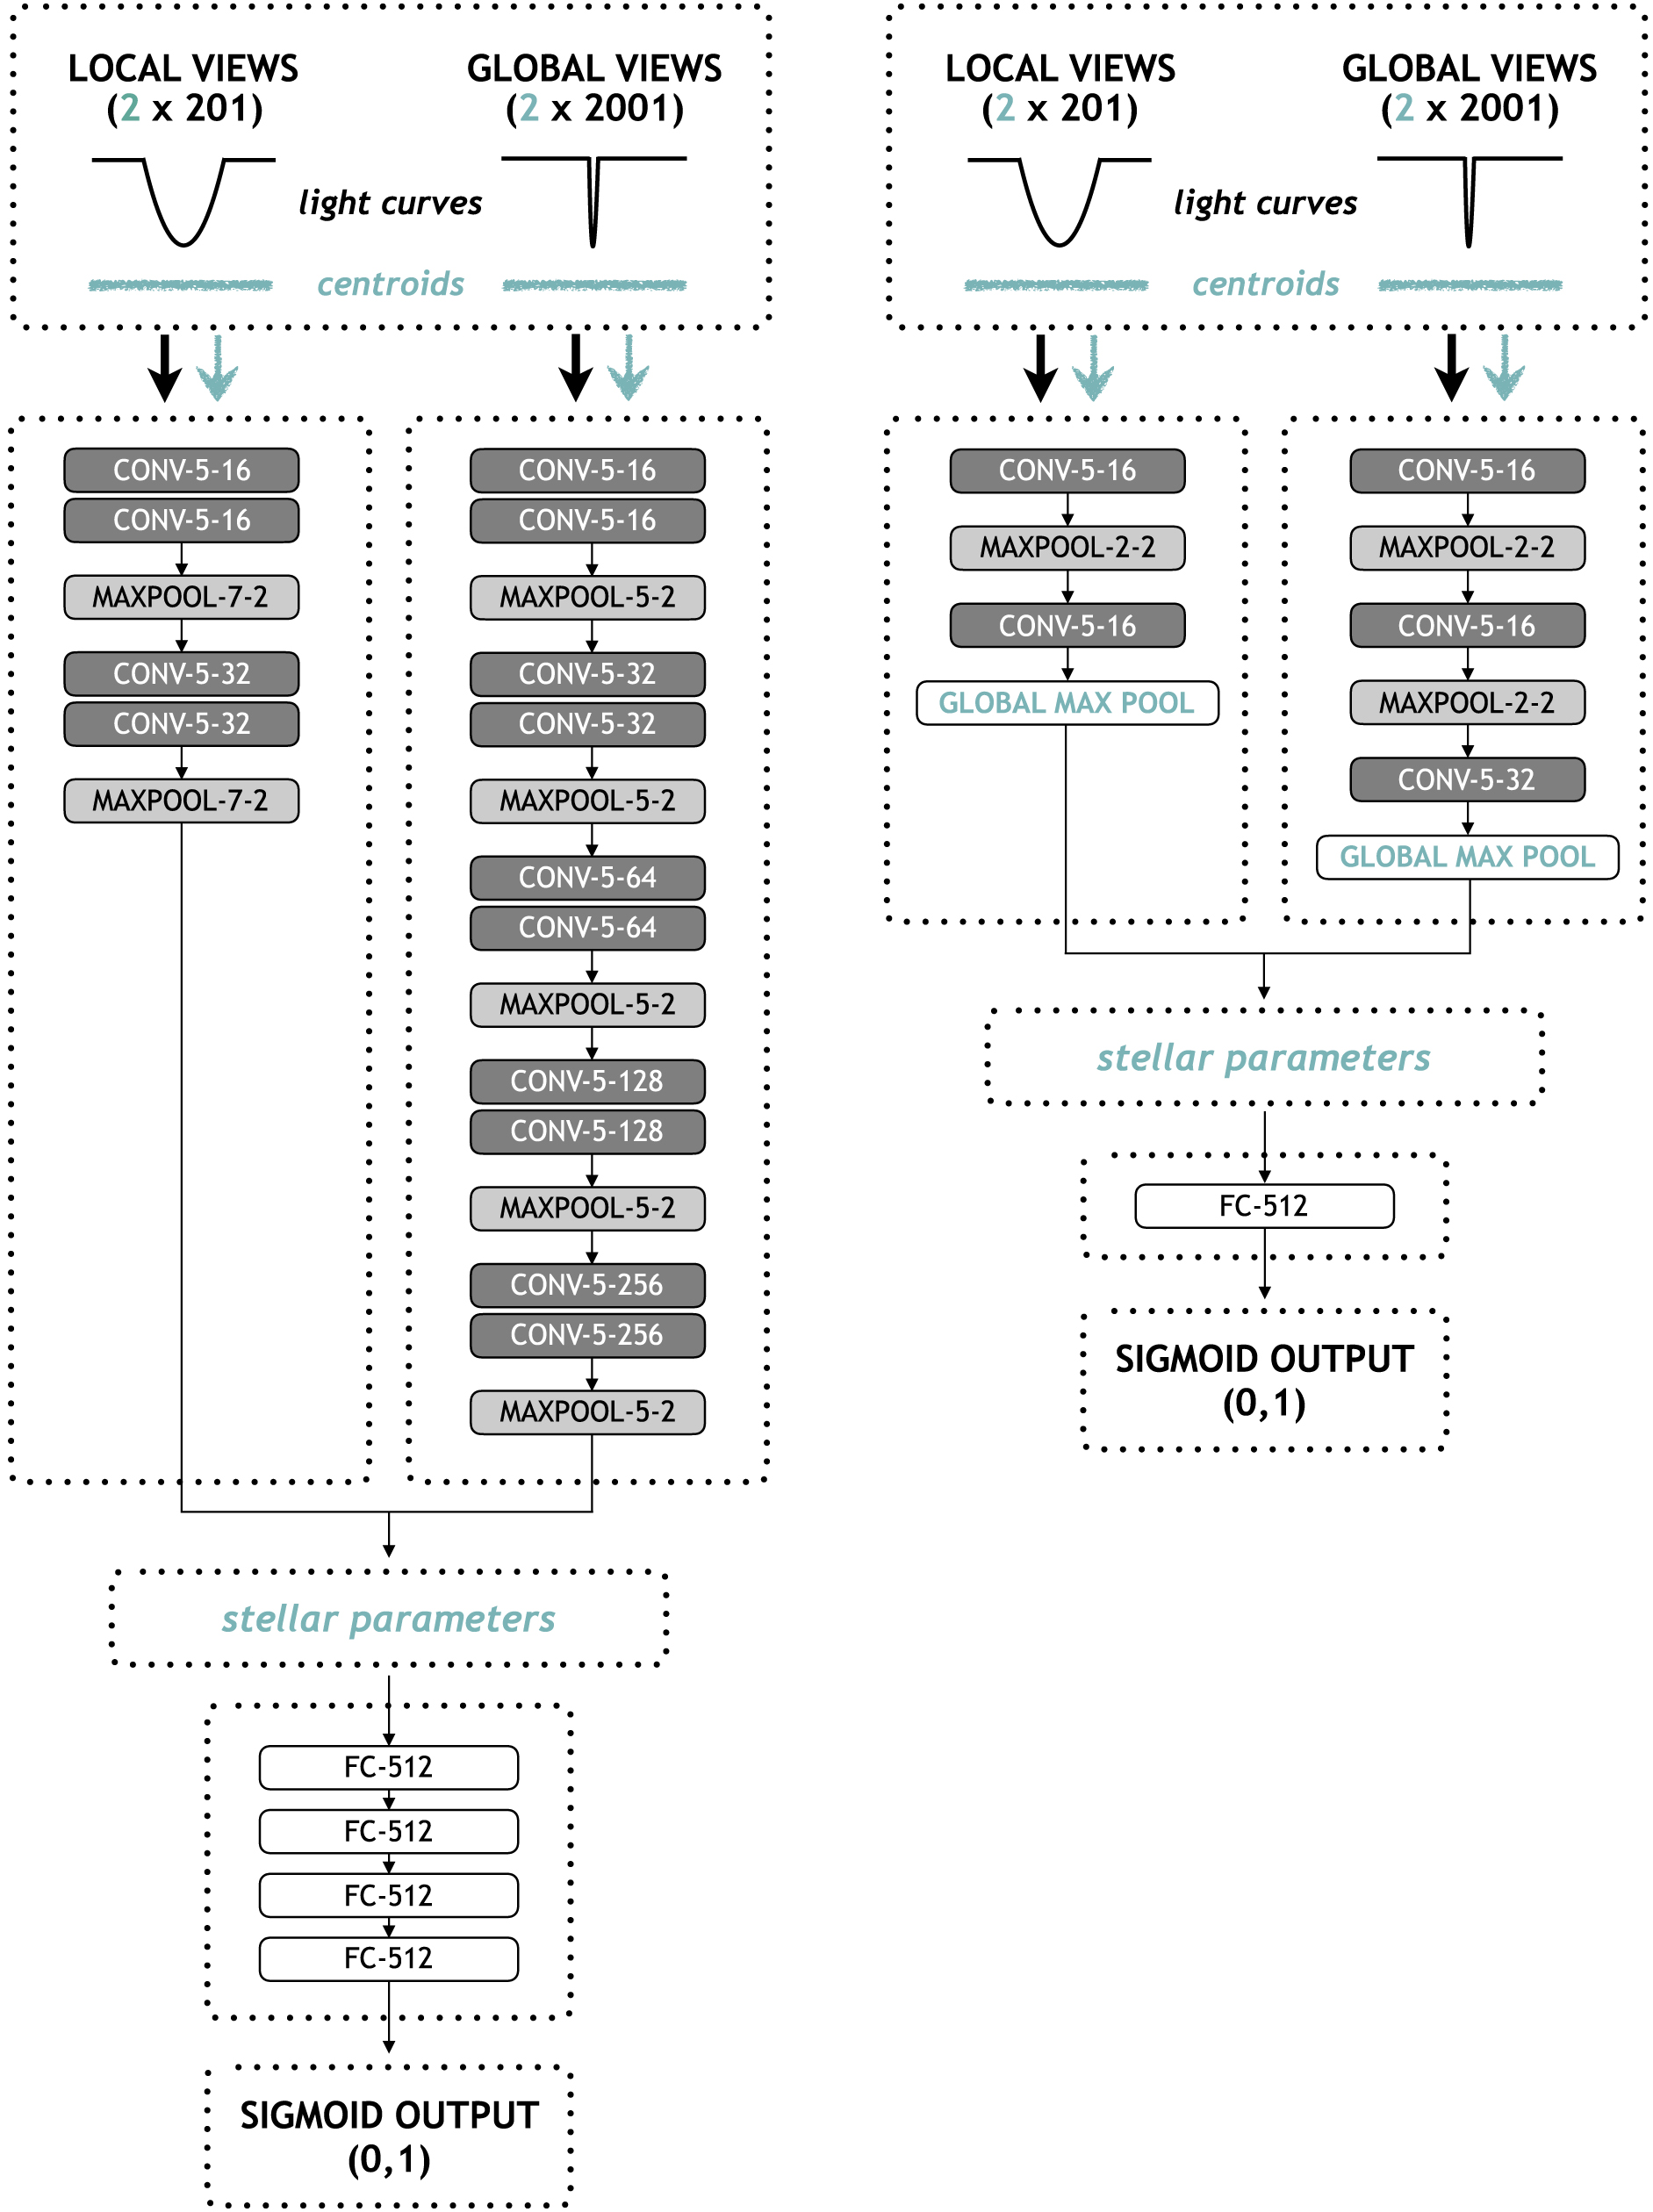
\includegraphics[scale=0.48]{Images/Ansdell.jpg}
    \caption{Exonet model additions are shown in Blue over the backbone Astronet model on the left while reduced XS models are shown on the right. The convolutional layers are denoted as CONV-〈kernel size〉-〈number of feature maps〉, the max pooling layers are denoted as MAXPOOL-〈window length〉-〈stride length〉, and the fully connected layers are denoted as FC-〈number of units〉. Source: Ansdell et al. (2018) \cite{exonet}}
    \label{fig:Ansdell}
\end{figure}